% !TeX spellcheck = de_DE_frami
%%%%%%%%%%%%%%%%%%%%%%%%%%%%%%%%%%%%%%%%%%%%%%%%
% COPYRIGHT: (C) 2012-2015 FAU FabLab and others
% Bearbeitungen ab 2015-02-20 fallen unter CC-BY-SA 3.0
% Sobald alle Mitautoren zugestimmt haben, steht die komplette Datei unter CC-BY-SA 3.0. Bis dahin ist der Lizenzstatus aller alten Bestandteile ungeklärt.
%%%%%%%%%%%%%%%%%%%%%%%%%%%%%%%%%%%%%%%%%%%%%%%%

\newcommand{\basedir}{fablab-document}
\documentclass{\basedir/fablab-document}

\usepackage{amssymb} % Symbole für Knöpfe
\usepackage{subfigure,caption}
\usepackage{eurosym}
\usepackage{textcomp} % \textcelsius
\usepackage{tabularx} % Tabellen mit bestimmtem Breitenverhältnis der Spalten
\usepackage{wrapfig} % Textumlauf um Bilder
\usepackage{float} % Ermöglicht H als Platzierungsoption
\usepackage{qrcode}
\renewcommand{\texteuro}{\euro}
\newcommand{\fachbegriff}[1]{(\textit{#1})}
\newcommand{\ra}{$\Rightarrow$}

% \linespread{1.2}
% \fancyhead{}
\date{\today}
\author{kontakt@fablab.fau.de}
\title{Einweisung 3D-Drucker}

\begin{document}

\maketitle
\begin{center}
	Für die 3D-Drucker \textbf{BambuLab P1S}, \textbf{Ultimaker-2+} und \textbf{Ultimaker-3}
\end{center}

\textbf{Nur eingewiesene Benutzer dürfen den Drucker selbstständig benutzen}, um  Beschädigungen zu vermeiden. Wenn du noch nicht eingewiesen bist, frage einen Betreuer. Er erklärt dir die eigenständige Bedienung. Wenn du alles verstanden hast, darfst auch du dann die Einweisung unterschreiben und den Drucker in Zukunft selbstständig verwenden.

\section{Regeln und Hinweise}
Für die Benutzung ist es wichtig, dass du folgende Hinweise beachtest:

\begin{itemize}
 \item Obwohl der 3D-Druck unter den Begriff 'Rapid Prototyping' fällt, kann ein Druck je nach Größe und Genauigkeit mehrere Stunden dauern. Die Software gibt nach dem Slicen einen Schätzwert für die Dauer an.
 \item Nicht unbeaufsichtigt drucken, vor allem am Anfang immer wieder nachschauen.\
Wenn du nicht bis zum Ende des Drucks da sein kannst, frage vorher einen Betreuer und hinterlasse einen Zettel mit deinem Namen und deinen Kontaktdaten.
   \item Der \textbf{Extruder wird bis zu 280°C heiß!} Zu deiner eigenen Sicherheit nicht direkt berühren.
 \item Drucker ausschalten,
 \begin{itemize}
  \item wenn der Drucker grobe Fehler macht 
  \item sehr untypische Geräusche macht
  \item sich der Ein-/Ausschalter befindet
  \begin{itemize}
   \item beim Ultimaker-2+ hinten links am Gehäuse
   \item beim Ultimaker-3 hinten rechts am Gehäuse
   \item beim BambuLab P1S hinten rechts am Gehäuse
  \end{itemize}
 \end{itemize}
 \item \textbf{Keine Schaber, Messer oder ähnliches verwenden} um Objekte von der Plattform zu entfernen
 \item Nichts manuell am Drucker bewegen. Dazu gibt es die Option Manuelles Verfahren auf dem Gerätedisplay.
 \item Materialwechsel und andere Wartungsarbeiten dürfen nur zusammen mit einer Aufsichtsperson durchgeführt werden.
 \item \textbf{Wiegen und Bezahlen nicht vergessen!}
\end{itemize}

\newpage
% % % % % % % % % % % % % % % %

\renewcommand{\contentsname}{Inhaltsverzeichnis / Arbeitsablauf}
\setcounter{tocdepth}{2}
\tableofcontents
\newpage

% % % % % % % % % % % % % % % %
\section{3D-Modell erstellen}
\subsection{Dateiformat}

Im STL-Dateiformat, Einheit: Millimeter. Alle gängigen 3D-Programme haben einen STL-Export.

\begin{itemize}
\item auf \href{https://thingiverse.com}{Thingiverse.com} gibt es viele vorgefertigte Modelle, als
Grundlage oder gleich zum fertig ausdrucken.
\item oder erstelle es mit einem Programm deiner Wahl
\begin{table}[H]
\centering
\begin{tabularx}{\textwidth}{|l|X|}
\hline \textbf{Name} & \textbf{Beschreibung} \\
\hline \multicolumn{2}{|c|}{\textit{kostenlose Software}}  \\
\hline Blender & relativ komplex aber auch für Freiformflächen geeignet  \\
\hline OpenSCAD & Skriptsprache für Konstruktion aus geometrischen Grundkörpern \\
\hline DesignSpark Mechanical & Angelehnt an professionelle CAD-Software, aber relativ einfach zu bedienen  \\
\hline TinkerCAD & sehr einfach, für Kinder gut geeignet  \\
\hline Google SketchUp & wenig Einarbeitung, geringer Funktionsumfang, für einfache Teile \\
\hline & \\
\hline \multicolumn{2}{|c|}{\textit{kostenpflichtige Software (proprietär)}}  \\
\hline PTC Creo, Solid Edge, Siemens NX & kostenlos beim RRZE für Studenten, professionelle Software \\
\hline Autocad Inventor & kostenlos bei Autodesk für Studenten ebenfalls für professionelle Anwendungen \\
\hline
\end{tabularx}
\end{table}
\item Die 3D-Daten müssen bestimmten Regeln entsprechen. Bei Modellierungsprogrammen wie Blender ist etwas Vorsicht bzw. Nacharbeit nötig, die meisten Konstruktionsprogramme (Solid Edge und Co., auch OpenSCAD) machen es prinzipbedingt von selbst richtig. Zu den Einschränkungen von Blender gibt es am Ende der Anleitung weitere Informationen.
\end{itemize}

\subsection{Einschränkungen der Formen}
\begin{itemize}
\item \textbf{Maximale Abmessungen}
\begin{itemize}
 \item Ultimaker-2+: L:223 B:220 H:205mm
 \item Ultimaker-3: L:215 B:215 H:200mm
 \item BambuLab P1S: L:256 B:256 H:256mm
\end{itemize}
\item Durch das Druckverfahren sind gewisse Formen schlecht druckbar. Oft ist Ausprobieren angesagt.
\item Um auch \enquote{schwierige} Formen drucken zu können, kann die Software \textbf{Stützstrukturen} erzeugen. Wenn diese Option aktiviert ist, erzeugt der Drucker unter Überhängen und Brücken ein loses Geflecht, das nach dem Drucken mit einer Zange oder einem Skalpell entfernt werden kann. Auf diese Weise können diese Einschränkungen umgangen werden. Nachteil ist die schlechtere Oberflächenqualität und der höhere Nachbearbeitungsaufwand.
\end{itemize}

\subsubsection{Drucken ohne Stützstruktur}
In diesem Abschnitt wird kurz beschrieben, welche Formen sich auch ohne Stützkonstruktion besonders gut bedrucken lassen. Wenn es ohne großen Aufwand möglich ist, sollten die Konstruktionen von vornherein so gewählt werden, dass sie gut bedruckbar sind.
\begin{center}
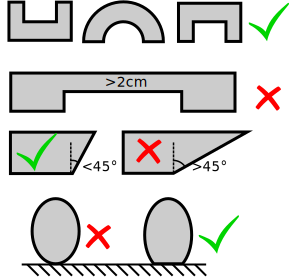
\includegraphics{./zeichnungen/formen.pdf}
\end{center}
\begin{itemize}
\item Überhänge sollten nicht zu groß sein
(Empfehlung\,{\textless}\,60$^\circ$)
\item Brücken sollten nicht zu weit sein (Empfehlung\,{\textless}\,20mm)
\item Das Objekt sollte mit ausreichend großer Fläche plan auf dem Boden aufliegen
\item Der untere Teil des Objekts sollte immer eine stabile Unterlage für die darüberliegenden Schichten bilden. (Den Eiffelturm sollte man also nicht auf dem Kopf stehend drucken.)
\end{itemize}
\newpage

% % % % % % % % % % % %

\section{Vorbereitung}

\subsection{Reinigung} \label{Reinigung}

Spätestens bei sichtbaren Verschmutzungen (Staub o.ä. auf der Druckplattform) oder schlechten Druckergebnissen.

\begin{itemize}
 \item Bodenplatte mit Papiertuch und Oberflächenreiniger reinigen
 \item Kunststoffabfälle aus PLA und leere Filamentspulen werden von uns recycelt, daher bitten wir Sie, diese Reste in den Behälter auf der rechten Seite des Druckers zu werfen.
\end{itemize}

\subsection{Material}
Im Fablab wird ausschließlich mit PLA gedruckt. Andere Materialien werden zu einem späteren Zeitpunkt angeboten.

\subsection{Materialwechsel}
Wir haben verschiedene Farben von PLA auf Lager. Wenn du eine andere möchtest, frag einfach nach.
Ein Materialwechsel an einem \textbf{Ultimaker} sollte jedoch nur von einem Betreuer durchgeführt werden. 

Für einen Materialwechsel beim \textbf{Bambu P1S} kann dies in der Software 'OrcaSlicer' ausgewählt werden. Hier stehen durch das proprietäre AMS - \textit{Automatic Material System} - insgesamt vier verschiedene Materialien für einen Druck zur Verfügung, entweder als Mehrfarbendruck oder wie gewohnt als Einfarbendruck. 

Besonders hervorzuheben ist, dass durch den Einsatz des AMS auch Filamente fast vollständig ausgenutzt werden können. Ist eine Farbe leer, kann nahtlos auf eine andere Rolle der gleichen Farbe/Materialart zugegriffen werden, so dass der Druck nicht beeinflusst wird. Dazu muss das AMS jedoch richtig eingestellt sein. 

Weitere Informationen zum Materialwechsel und zur Einstellung für den Betreuer $\to$ \ref{Materialwechsel})

\newpage
% % % % % % % % % % % %

\section{3D-Modell für den Druck vorbereiten}

Damit ein 3D-Modell gedruckt werden kann, muss es in Schichtbilder übersetzt werden, die der Drucker nach und nach zu einem dreidimensionalen Objekt zusammensetzt. Dazu verwenden wir sowohl für den Ultimaker als auch für den Bambu P1S eine Slicer-Software namens \textit{OracSlicer}.

\vspace{2em}

\begin{figure} [H]
	\centering
	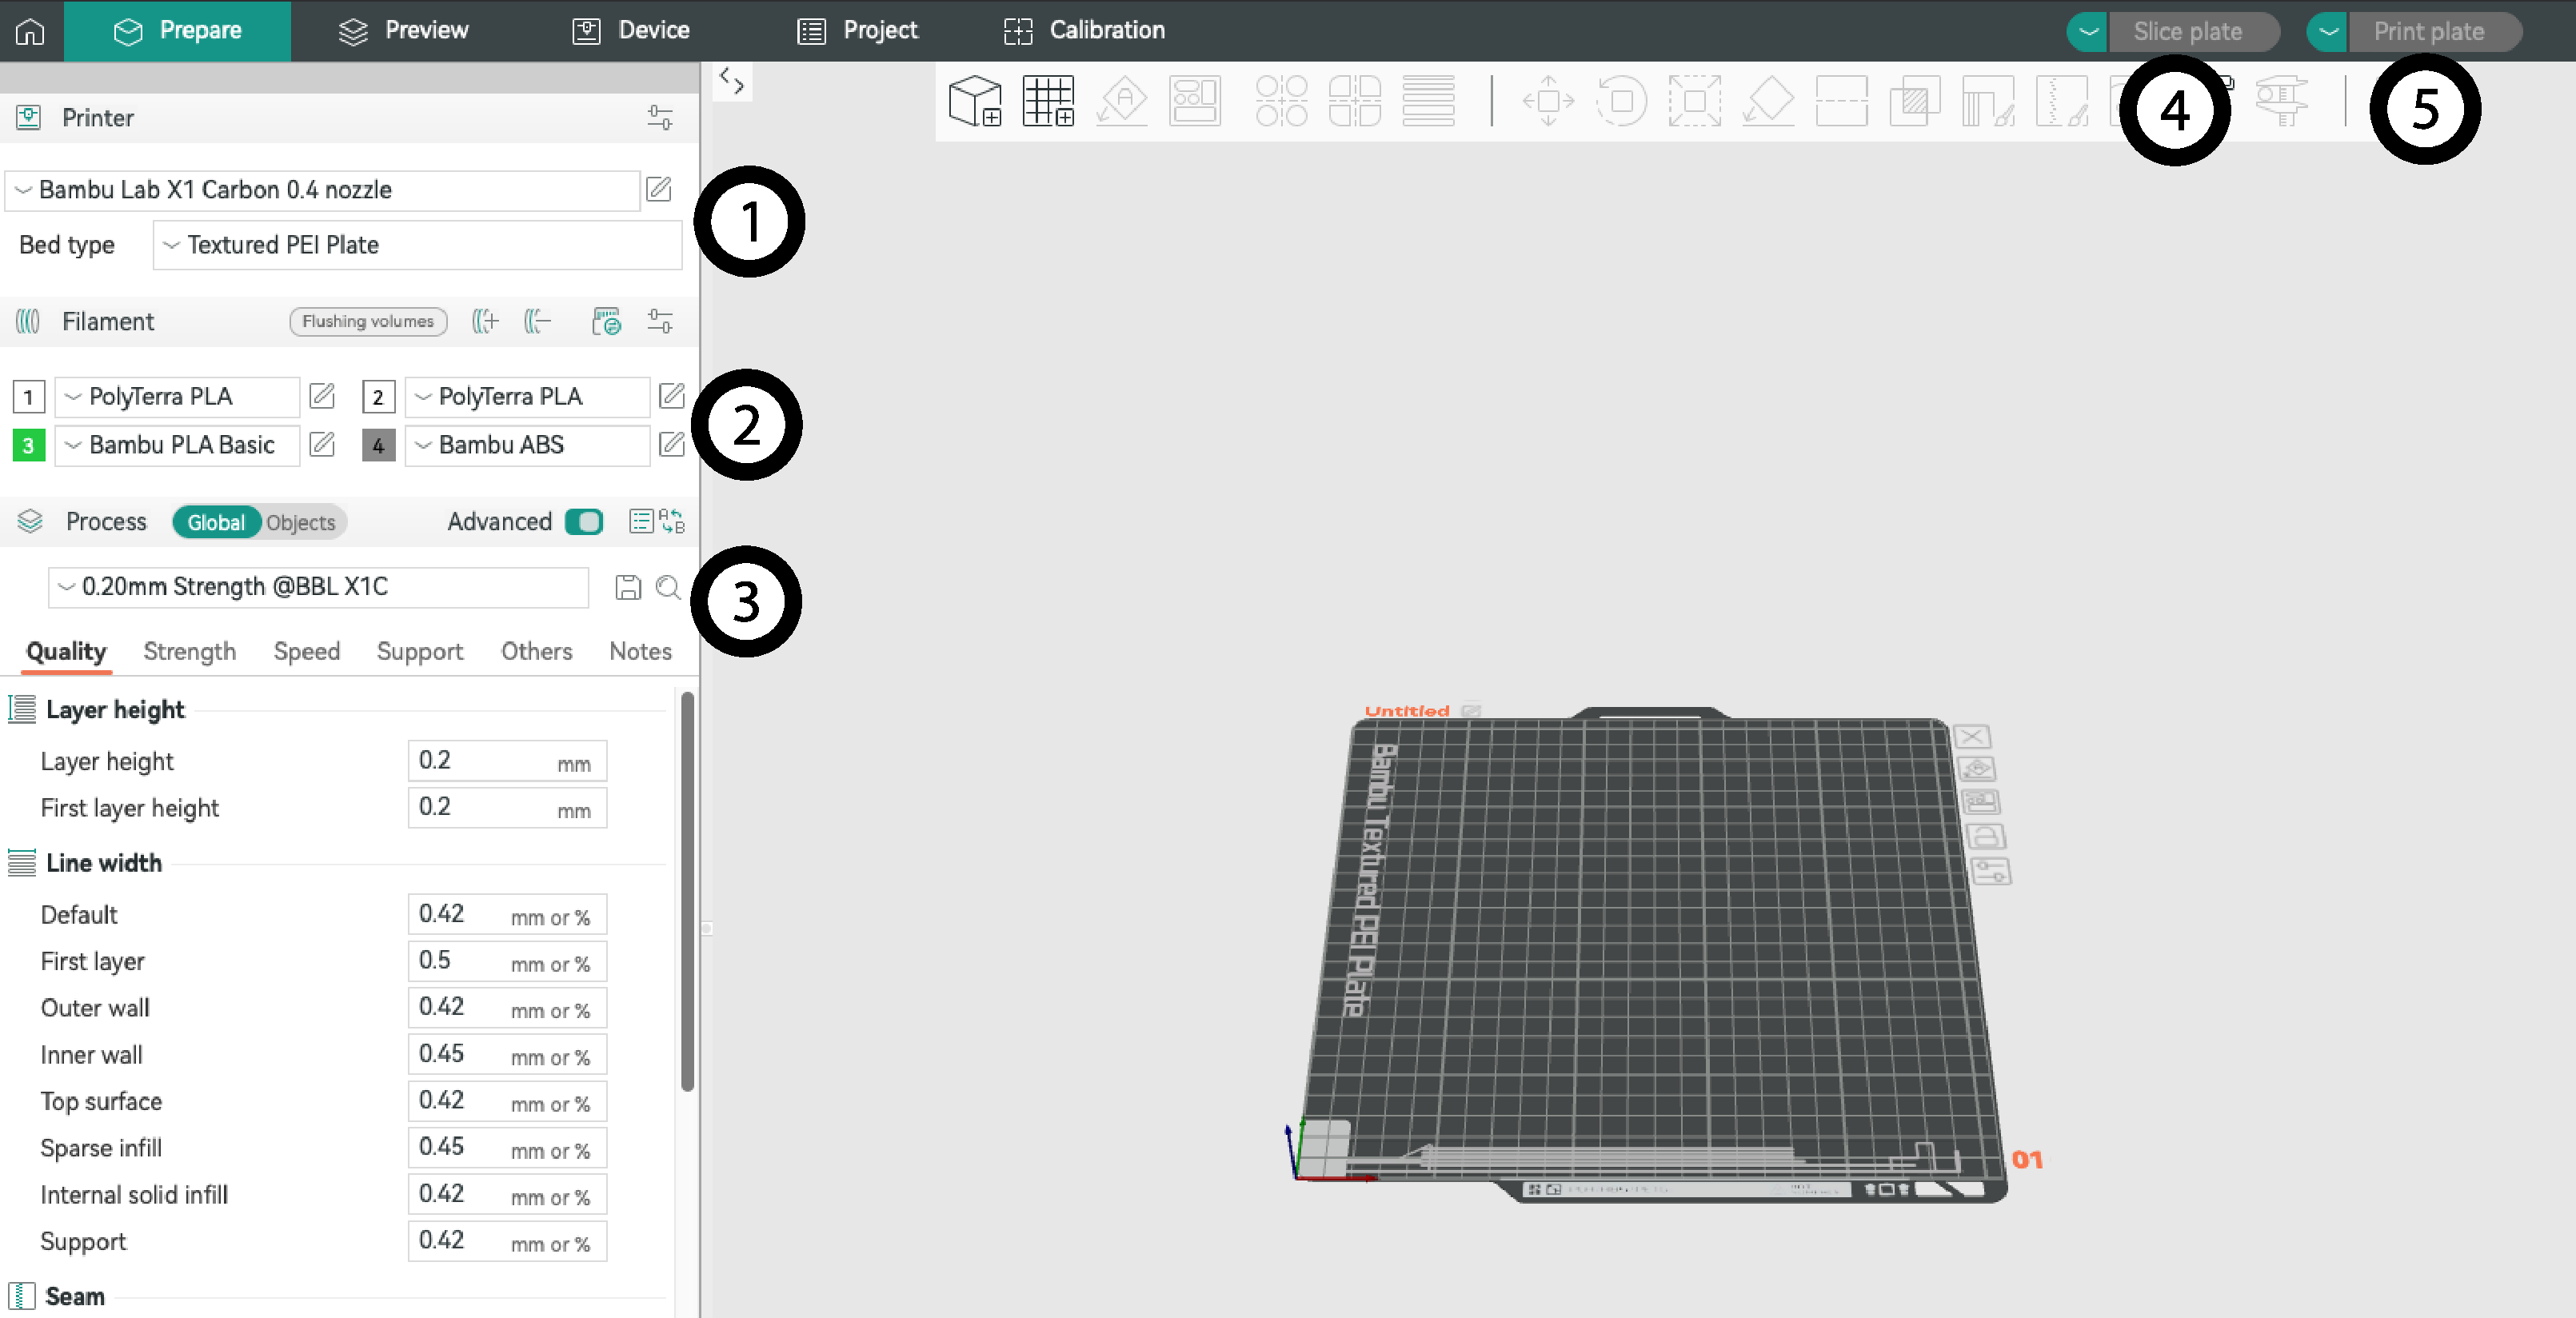
\includegraphics[width=1.0\textwidth]{./zeichnungen/OrcaSlicer.pdf}
	\caption{Menüführung von OrcaSlicer. Druckerauswahlmenü \large\textcircled{\normalsize \texttt{1}}, Filamentauswahlmenü \large\textcircled{\normalsize \texttt{2}}, Auswahltder Qualitätsstufe \large\textcircled{\normalsize \texttt{3}}, Bauraum Slicen \large\textcircled{\normalsize \texttt{4}}, Bauraum exportieren \large\textcircled{\normalsize \texttt{5}} }
	\label{abb.Grafik1}
\end{figure}

\vspace{2em}

\begin{itemize}
\item Ziehen Sie die STL/STEP-Datei einfach per Drag-and-Drop in das \textit{OrcaSlicer}-Fenster. Auf diese Weise können auch mehrere Dateien hinzugefügt werden.
\item Das Objekt auf einer bestimmten Seite platzieren, skalieren, verschieben, drehen etc. wie gewünscht. Verwenden Sie dazu die Schaltflächen in der weißen Menüleiste über dem Bauraum.
\item Den richtigen Drucker in der linken Menüleiste auswählen \large\textcircled{\normalsize \texttt{1}} (Ultimaker Ultimaker-2+, Ultimaker-3 oder BambuLab P1S)
\item Stellen Sie sicher, dass in der linken Menüleiste \large\textcircled{\normalsize \texttt{2}} PLA als Material ausgewählt ist.\\Bei BambuLabs P1S kann mit einem Rechtsklick auf das Objekt im erscheinenden Kontextmenü das verwendete Filament geändert werden. Achtung, Mehrfarbendrucke erzeugen ein zusätzliches Objekt auf dem Bauraum, um die Düse zu reinigen. 
\item Im Druckqualitätsmenü \large\textcircled{\normalsize \texttt{3}} eine geeignete Qualitätsstufe wählen. Empfohlen werden Sandart 0,20mm und Strenght 0,20mm. Die anderen Qualitätsstufen dauern nur wesentlich länger, wenn es um Qualitätsverbesserungen geht. 
\item Gegebenenfalls sind Stützkonstruktionen erforderlich, wählen Sie dazu in der linken Seitenleiste das Menü \textit{Support} und setzen Sie das Häkchen bei aktiviert. Es stehen die Optionen \textit{Normal} oder \textit{Baum} für die Art der Stützkonstruktionen zur Verfügung. \textit{Baum} eignet sich sehr gut für organische Strukturen, während \textit{Normal} eher für technische Objekte mit klaren Kanten von Vorteil ist. 
\item Durch Klicken auf den Slice-Button \large\textcircled{\normalsize \texttt{4}} kann die Umrechnung des Bauraums für die Maschine ausgelöst werden. 
\item Erst nach einem Export der Datei auf ein Speichermedium kann der Drucker mit Daten versorgt werden. Wählen Sie dazu den Export Button \large\textcircled{\normalsize \texttt{5}} mit "Gesamten Bauraum als GCode exportieren" drücken und auf ein Speichermedium (SD für Ultimaker-2+ und Bambu P1S bzw. USB-Stick für Ultimaker-3) speichern.
\item Stecken Sie die SD-Karte in den Kartenleser (Ultimaker-2+ oder Bambu P1S) oder den USB-Stick (Ultimaker-3). Beim Bambu kann es erforderlich sein, den MicroSD-Adapter aus- und wieder einzustecken, damit er erkannt wird. 
\item Über das OnScreen Menü kann nun die Datei zum Drucken ausgewählt und gedruckt werden. 
\end{itemize}

\section{Bezahlen und abschließen}

Das Objekt vorsichtig von der Platte lösen. Meistens kann es von Hand gelöst werden. Wenn nicht
warten, bis die Platte etwas abgekühlt ist. \textbf{Nicht versuchen, das Objekt mit scharfen oder spitzen Gegenständen herunterzuhebeln!}

Wiegen Sie das Objekt mit einer Feinwaage (in der Regel bei 3D-Druckern vorhanden), der Preis pro Gramm wird in das Kassensystem eingegeben.

Alles muss gewogen werden, auch die Stützstruktur. 
\textbf{Fehldrucke müssen ebenfalls bezahlt werden.}

\pagebreak

% % % % % % % % % % % % % % %

\section{Infos für Experten}

\subsection{Kurze Einführung in die wichtigsten Fachbegriffe bei STL:}

\begin{itemize}
\item Einheit \fachbegriff{unit}: Länge, die der Zahl „1“ entsprechen soll (bei uns
1 Millimeter)
\item Punkt \fachbegriff{vertex}: Stelle im Raum
\item Kante \fachbegriff{edge}: Verbindungslinie zwischen zwei Punkten
\item Fläche \fachbegriff{face}: Dreieck, das zwischen drei Punkten bzw. zwei
benachbarten Kanten aufgespannt wird. Im verwendeten STL-Dateiformat
gibt es nur Dreiecksflächen. Krümmungen werden aus vielen
Dreiecksflächen angenähert.
\item Polygonnetz \fachbegriff{mesh}: Gesamtheit aller Flächen, die einen Körper
ergibt. Alles innerhalb des Netzes soll mit Kunststoff gefüllt werden,
alles außerhalb ist Luft.
\end{itemize}

\subsection{Einschränkungen bei Blender und manchen anderen Programmen} \label{lowlevel-einschraenkungen}

Das 3D-Modell muss gewisse Einschränkungen erfüllen, damit die Drucksoftware es versteht. Da man mit Tools wie Blender auch unsinnige Dinge bauen kann (Modelle mit Löchern, unlogische Dinge bei denen innen und außen nicht eindeutig ist), muss auf folgendes geachtet werden.
\begin{itemize}
\item Wasserdicht: Der Körper muss rundum geschlossen sein, er darf keine
Löcher aufweisen,  die Hülle muss ein zusammenhängendes Netz sein.
\item Polygonnetz \fachbegriff{mesh} schneidet sich nicht selbst: Verschiedene
Körper dürfen sich nicht überlappen. Sie müssen stattdessen zu einem
Körper vereinigt werden. In Blender geht dies zum Beispiel mit dem
Boolean Modifier.
\item Mannigfaltig \fachbegriff{manifold}: Dieser Begriff ist schwierig zu
beschreiben. Vereinfacht gesagt dürfen zu jeder Kante nur zwei Flächen
gehören. Es dürfen also zum Beispiel keine Flächen innerhalb eines
Körpers existieren.
\end{itemize}

% % % % % % % % % % % % % %

\newpage

\section{Infos für Betreuer}

\subsection{Filamentwechsel}\label{filamentwechsel}

\subsubsection{Ultimaker-2+}
\begin{itemize}
    \item ''Material'' \ra ''Change''; Anweisungen im Display beachten
    \item Drucker heizt vor und fährt dann das Filament zurück
    \item Filament hinten vorsichtig entnehmen; nicht verknoten oder brechen!
    \item neues Filament auf Spindel und ''Ready'' drücken
    \item neues Filament einführen bis Fördermotor zieht; aufpassen dass Filament sich nicht verknotet!
    \item ''Ready'' drücken; Drucker fährt Filament vor und extrudiert
    \item wenn er schön extrudiert, nochmal drücken und das eingelegte Filament wählen
\end{itemize}


\subsection{Ausrichten der Buildplate}

\subsubsection{Ultimaker-2+}
\begin{itemize}
\item Extruder reinigen, dass sich kein Rest zw. Buildplate und Extruder befindet
\item Assistent: ''maintenance'' \ra ''buildplate''
\item den Anweisungen auf dem Display befolgen
\item man muss mal mit dem Rad und den Steppern, mal manuell mit den Schrauben die Buildplate leveln (zuerst auf 1mm, dann mit einem Blatt Papier)
\end{itemize}


\subsection{Ultimaker demontieren und putzen}
Lasse es dir vorher von jemand mit Ahnung zeigen! Nur durchführen wenn unbedingt nötig.

Die Düse bitte nicht mit einem Metallstück freistochern, da hierdurch nur die Oberfläche verkratzt wird und die Düse nur noch schlechter funktioniert. Es ist möglich, fest sitzenden Dreck mit einem Stück Filament durchzudrücken. Dazu nimmt man sich ein Stück Filament und drückt es mit ausreichend Kraft durch den heißen Extruder. Eine Kombizange hilft. Dabei nicht abrutschen oder den Extruderkopf überlasten.
\\

Eine Anleitung zum Wechseln der Düse beim Ultimaker 2+: 
 \\ https://support.makerbot.com/s/article/1667411296273 \hspace{2cm}
\qrcode[height=2cm]{https://support.makerbot.com/s/article/1667411296273}

\vspace{1cm}

Beim Ultimaker 3 kann die Düse nicht einzeln gewecheselt werden. Hier müssen die ganzen Printcores getauscht werden.

\subsection{Pflege \& Wartung}

\begin{itemize}
\item Achsen sollten regelmäßig gefettet werden (1x monatlich)
\item Riemenspannung und Riemenzustand überprüfen
\item die Ausrichtung und den Zustand der Buildplate überprüfen
\end{itemize}

\ccLicense{3d-drucker-einweisung}{Einweisung 3D-Drucker}

\end{document}